%%%%%%%%%%%%%%%%%%%%%%%%%%%%%%%%%%%%%%%%%%%%%%%%%%%%%%%%%%%%%%%%%%%%%%%%%%%%%%%%%%
\begin{frame}[fragile]\frametitle{}
\begin{center}
{\Large RAG in Production}
\end{center}
\end{frame}


%%%%%%%%%%%%%%%%%%%%%%%%%%%%%%%%%%%%%%%%%%%%%%%%%%%%%%%%%%%%%%%%%%%%%%%%%%%%%%%%%%
\begin{frame}[fragile]\frametitle{}
\begin{center}
{\Large Vector DB in Production}

{\tiny (Ref; LinkedIn post by Nirant Kasliwal)}
\end{center}
\end{frame}


%%%%%%%%%%%%%%%%%%%%%%%%%%%%%%%%%%%%%%%%%%%%%%%%%%%%%%%%%%%%%%%%%%%%%%%%%%%%%%%%%%
\begin{frame}[fragile]\frametitle{The Problem}
\begin{itemize}
    \item Vector search choices often spark endless technical debates.
    \item Teams struggle to balance speed, quality, and cost.
    \item Poor decisions stem from unclear priorities.
\end{itemize}
\end{frame}

%%%%%%%%%%%%%%%%%%%%%%%%%%%%%%%%%%%%%%%%%%%%%%%%%%%%%%%%%%%%%%%%%%%%%%%%%%%%%%%%%%
\begin{frame}[fragile]\frametitle{The Tradeoff Triangle}
\begin{itemize}
    \item Vector search is a balance of:
    \begin{itemize}
        \item Speed (low latency)
        \item Quality (high recall)
        \item Cost (infrastructure)
    \end{itemize}
    \item You can only optimize two; the third will suffer.
    \item Overpromising all three leads to failure.
\end{itemize}
\end{frame}

%%%%%%%%%%%%%%%%%%%%%%%%%%%%%%%%%%%%%%%%%%%%%%%%%%%%%%%%%%%%%%%%%%%%%%%%%%%%%%%%%%
\begin{frame}[fragile]\frametitle{Why a Decision Framework Helps}
\begin{itemize}
    \item Avoids circular discussions.
    \item Focuses on business needs, not technical preferences.
    \item Saves time and clarifies tradeoffs.
\end{itemize}
\end{frame}

%%%%%%%%%%%%%%%%%%%%%%%%%%%%%%%%%%%%%%%%%%%%%%%%%%%%%%%%%%%%%%%%%%%%%%%%%%%%%%%%%%
\begin{frame}[fragile]\frametitle{Concrete Questions Over Abstract Debates}
\begin{itemize}
    \item Is cost a hard constraint?
    \item Do we need latency under 50ms?
    \item What recall can users actually perceive?
\end{itemize}
\end{frame}

%%%%%%%%%%%%%%%%%%%%%%%%%%%%%%%%%%%%%%%%%%%%%%%%%%%%%%%%%%%%%%%%%%%%%%%%%%%%%%%%%%
\begin{frame}[fragile]\frametitle{A Real-World Example}
\begin{itemize}
    \item Product team wanted ``Google recall'' + ``Stripe latency'' + startup budget.
    \item Framework helped align on priorities.
    \item Solution: quantized index optimized for user-impacting metrics.
\end{itemize}
\end{frame}

%%%%%%%%%%%%%%%%%%%%%%%%%%%%%%%%%%%%%%%%%%%%%%%%%%%%%%%%%%%%%%%%%%%%%%%%%%%%%%%%%%
\begin{frame}[fragile]\frametitle{Vector Search = Navigation}
\begin{itemize}
    \item Optimization is like choosing a GPS route.
    \item Fastest isn’t always best—consider tolls and risk.
    \item Decision tree guides you to the best compromise.
\end{itemize}
\end{frame}

%%%%%%%%%%%%%%%%%%%%%%%%%%%%%%%%%%%%%%%%%%%%%%%%%%%%%%%%%%%%%%%%%%%%%%%%%%%%%%%%%%
\begin{frame}[fragile]\frametitle{Vector Db Descion Tree}
		\begin{center}
		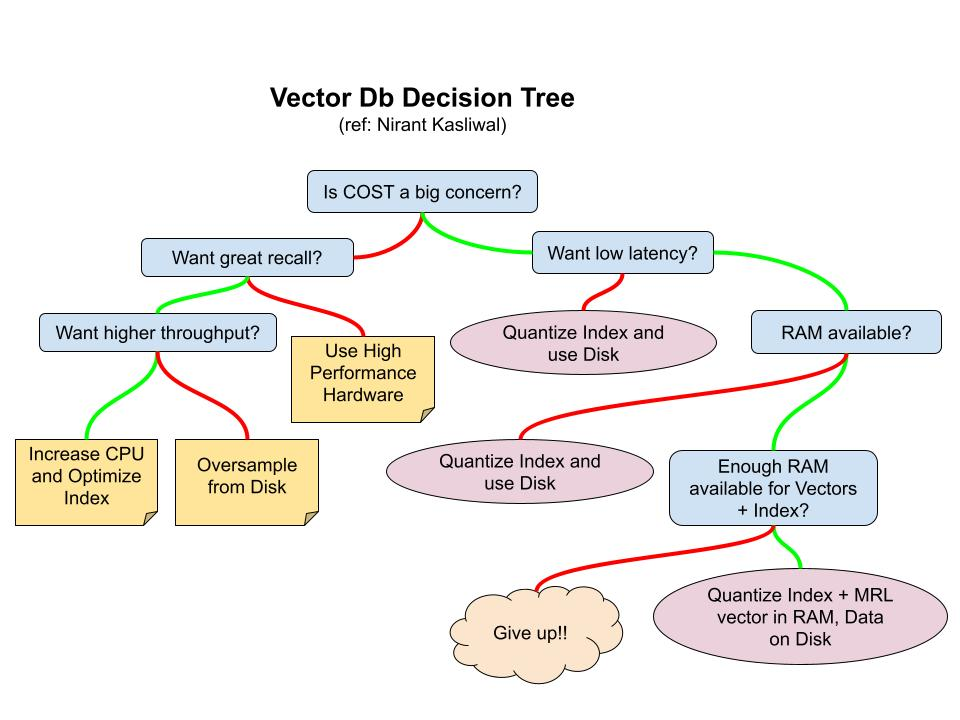
\includegraphics[width=\linewidth,keepaspectratio]{rag38}
		\end{center}
\end{frame}

%%%%%%%%%%%%%%%%%%%%%%%%%%%%%%%%%%%%%%%%%%%%%%%%%%%%%%%%%%%%%%%%%%%%%%%%%%%%%%%%%%
\begin{frame}[fragile]\frametitle{Key Takeaway}
\begin{itemize}
    \item Use structured questions to steer tradeoffs.
    \item Let business goals—not tech idealism—drive choices.
    \item This framework turns friction into clarity.
\end{itemize}
\end{frame}



